\documentclass[]{article}
\usepackage{amsmath}
\usepackage{graphicx}

\begin{document}

\section{Simulations}
OK, if I compare MSE for $\beta$ directly, it indeed cause the problem. Take 1/0 (\textbf{code 1}) vs. 1/-1 (\textbf{code 2}) as an example. Let the intercept and coefficient for categorical variable be $\beta_0$ and $\beta_c$ for \textbf{code 1}, while  $\beta'_0$ and $\beta'_c$ for \textbf{code 2}. Then $\beta'_0 = \beta_0 + \beta_c/2$ and $\beta'_c = \beta_c/2$. So the variance of $\boldsymbol{\breve{\beta}} - \hat{\boldsymbol{\beta}}_{MLE}$ for \textbf{code 2} will be smaller than \textbf{code 1}, because $\beta'_c = \beta_c/2$. This will lead to a lower MSE for \textbf{code 2}.

To fix that, I now compare the MSE for linear predictor, i.e. define MSE as $S^{-1}\sum_{s=1}^{S}\frac{||\boldsymbol{X}\breve{\boldsymbol{\beta}}^{(s)} - \boldsymbol{X}\hat{\boldsymbol{\beta}}_{MLE}||^2}{n - p}$

Now, To make the results more significant, I only include 1 continuous variable with one categorical variable with 2 levels. 

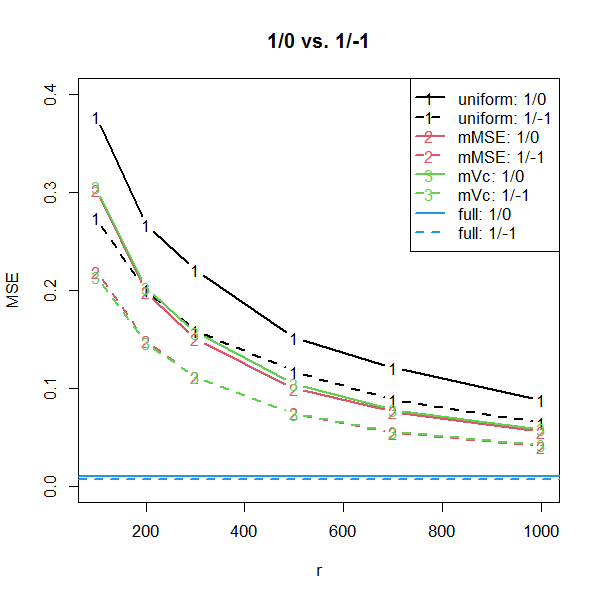
\includegraphics[width = .8\textwidth]{plot_2levels.png}

It seems that coding baseline as (-1, -1) is worse than coding as (0, 0). As we can imagine, coding the baseline with less absolute values will make things better. Here I use the same data, but code the baseline as (2, 2):

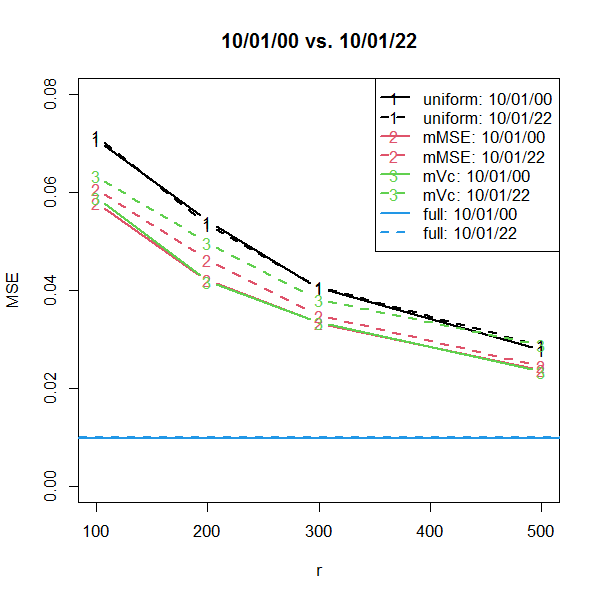
\includegraphics[width = .8\textwidth]{plot_2levels_2.png}

Now, it looks much worse, especially for L-optimization. (A-optimization is somewhat more robust to different coding, because of $\boldsymbol{M}_{X}^{-1}$ term)

\section{Recommendations}

Our goal is to suggest a best way for coding the categorical variable, to minimize bias in sub-sampling procedure.

Based on previous observations, we can see that if we code the variable with larger absolute value, it will lead to a larger bias. The L-optimization is more sensitive to the change of coding. Therefore, I would suggest to code the variable with least total absolute values (or the smallest Frobenius norm for dummy variable matrix (?)). However, this should not sacrifice the interpretability, for example coding as 0.5/0 will has less interpretation power than 1/0, although I guess 0.5/0 will give less bias.

To summarize, when we do sub-sampling, we should include as much 0 as possible in the coding. To be specific, assume the variable has L levels, I suggest use L-1 dummy variables as follows:\\


\begin{tabular}{|c|c|c|c|c|c|}
	\hline
	level& $X_1$& $X_2$&...&$X_{L-2}$&$X_{L-1}$\\
	\hline
	level 1 & 1 & 0 & ... & 0 & 0 \\
	\hline
	level 2 & 0 & 1 & ... & 0 & 0 \\
	\hline
	... & 0 & 0 & ... & 0 & 0 \\
	\hline
	level L-2 & 0 & 0 & ... & 1 & 0 \\
	\hline
	level L-1 & 0 & 0 & ... & 0 & 1 \\
	\hline
	level L & 0 & 0 & ... & 0 & 0 \\
	\hline
\end{tabular}
\\

The potential explanation: Consider about L-optimization SSP:
\begin{equation*}
	\pi_{i}^{mVc} = \frac{|y_i-p_i(\hat{\beta}_{MLE})||\boldsymbol{x}_i||}{\sum_{j=1}^{n}|y_i-p_i(\hat{\beta}_{MLE})||\boldsymbol{x}_i||}
\end{equation*}
If the dummy variable is coded as large absolute values, it will let the dummy variable guide the SSP, and this will cause bias?

	
\end{document}


